
\newpage
\section{Bilan radiatif en milieu transparent entre surfaces opaques}
L'objectif de cette partie est d'exprimer le flux radiatif $q$~[W/m²] sortant de chaque face solide, afin de prendre en compte le rayonnement dans les transferts thermiques. Plusieurs phénomènes sont à prendre en compte simultanément dans un problème radiatif: l'émission du système (qui suit la loi de Stefan Boltzmann) ainsi que la transmission, l'absorption et la réflexion de l'énergie irradiée. Plusieurs hypothèses courantes permettent de simplifier la définition des domaines physiques. La remise en cause de ces hypothèses ne rentre pas dans le cadre de ce travail, mais pourra nourrir la discussion d'un projet futur.


\subsection{Formulation du problème}
On considère ici que le rayonnement se fait entre des surfaces solides opaques au travers d'un milieu transparent. La première hypothèse est la transparence du fluide, i.e. il n'absorbe, n'émet ni réfléchi de rayonnement.


L'hypothèse d'opacité des surfaces permet de négliger la transmission dans ces milieux. Le rayonnement incident, aussi appelé l'irradiance ($G$~[W/m²]) est donc réfléchi ou absorbé. On obtient alors la complémentarité des coefficients de réflexion et d'absorption : $\forall \lambda, \, \rho_{\lambda} + \alpha_{\lambda} = 1$. On suppose ensuite que les surfaces sont grises: les coefficients $\alpha$ et $\epsilon$ sont indépendants de la longueur d'onde $\lambda$. La radiosité $J$~[W/m²] s'écrit alors comme la somme de la puissance émissive $E$~[W/m²] et de la réflexion de l'irradiance $\rho G$ : 
\begin{equation}
    \forall \vec{r}_i \in \text{Surface}_i, \quad J_i(\vec{r_i}) = \epsilon_i \sigma \big(T(\vec{r}_i)\big)^4 + \rho_i G_i(\vec{r_i})
\label{def:radiosite}
\end{equation} 

Avec $\epsilon_i$ (resp. $\rho_i$) l’émissivité (resp. la réflectivité) de la surface $i$, $\sigma$ désigne la constante de Stefan-Boltzmann et $T_i(\vec{r}_i$ la température de la surface $i$ à la position $\vec{r}_i$. La radiosité correspond à l'ensemble de l'énergie radiée qui quitte une surface. Le flux radiatif en surface peut ainsi s'écrire grâce à un  bilan comme représenté sur la Figure \ref{fig:radio}:
\begin{equation}
    \forall \vec{r}_i \in \text{Surface}_i,\quad q_i(\vec{r}_i) =  J(\vec{r}_i)  - G(\vec{r}_i) 
    \label{eq:qr}
\end{equation}

 Enfin, on suppose que l'irradiation et les surfaces sont diffuses. On a alors $G_{\lambda, i} (\lambda, \theta, \varphi)$ est indépendant de $\lambda$, $\theta$ et $\varphi$ et comme le montre la Figure \ref{fig:diffus}.

%\textit{Loi de Kirchhoff : alpha = espilon si isoT+ petit corps dans une cavité, eq thermique}

\begin{minipage}{0.45\textwidth}
    \centering
    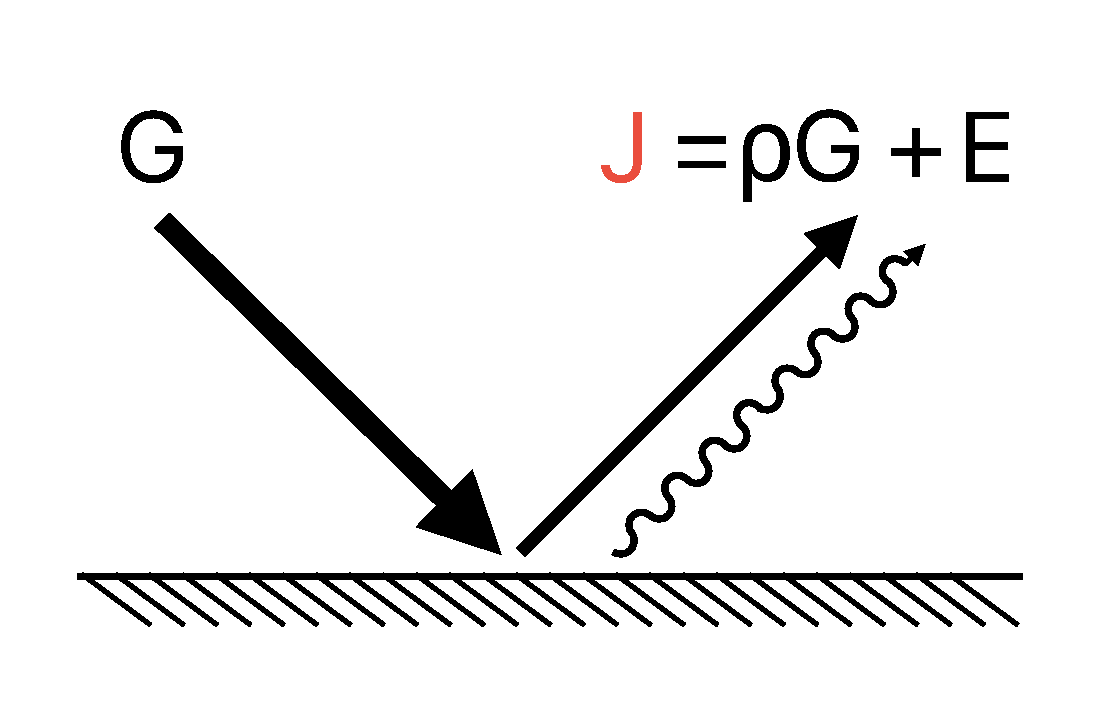
\includegraphics[width=0.9\linewidth]{PICTURES/radiosite.pdf}
    \captionof{figure}{Échanges radiatifs considérés dans le problème}
    \label{fig:radio}
\end{minipage}
\hfill
\begin{minipage}{0.45\textwidth}
    \centering
    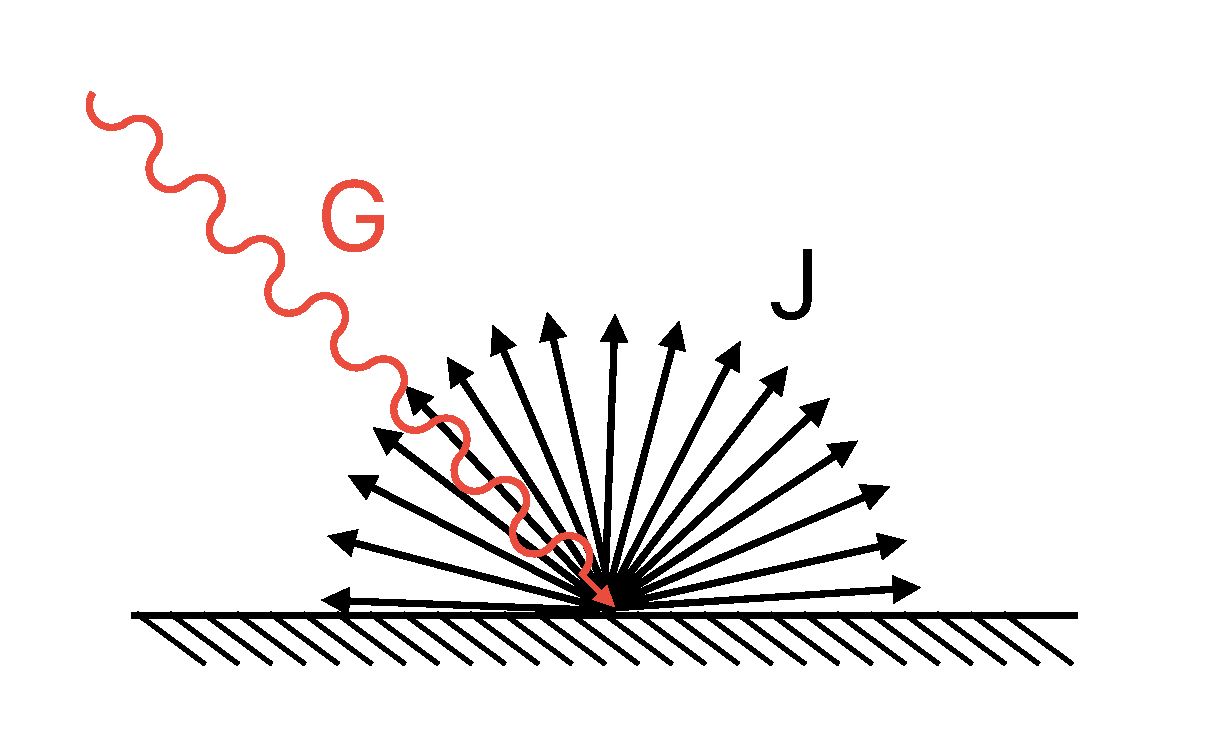
\includegraphics[width=0.9\linewidth]{PICTURES/diffus.pdf}
    \captionof{figure}{Illustration de l'hypothèse de réflexion et émission diffuse}
    \label{fig:diffus}
\end{minipage}





Pour finir, l’irradiance est exprimée conformément à la Figure \ref{fig:fij_schema} en fonction des radiosités sous la forme : 
\begin{equation}
    \forall i \in [1, n], \forall \vec{r_i} \in A_i , \quad G_i(\vec{r_i}) = \sum_{j = 1}^{n} \frac{1}{\pi} \int_{A_i} d^2(\vec{r_j})J_j(\vec{r_j})\bigg[\frac{cos(\theta_{ij})cos(\theta_{ji})}{||\vec{r_i}-\vec{r_j}||^2} \chi{(\vec{r_i},\vec{r_j})}\bigg] 
    \label{def:irra}
\end{equation}
Avec $\chi$ la fonction de visibilité (ou d'encaissement) qui vaut 1 si les points $\vec{r_i}$ et $\vec{r_j}$ sont visibles l'un de l'autre, et 0 sinon.
\begin{figure}[h]
    \centering
    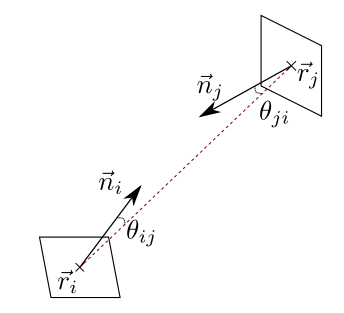
\includegraphics[width = 0.3\linewidth]{PICTURES/FIJ.png}
    \caption{Illustration des notations géométriques introduites à l'Eq \ref{eq:irra}}
    \label{fig:fij_schema}
\end{figure}

La connaissance des radiosités est donc capitale pour les transferts radiatifs.





